% ! TeX root = ./document.tex
\documentclass[9pt, aspectratio=169]{beamer}
% ! TeX root = ../document.tex
\usepackage[utf8]{inputenc}
\usepackage{multicol}
\usepackage{pgfpages}
\usepackage{roboto}
\usepackage{fontawesome5}
\usepackage[T1]{fontenc}
\usepackage[final]{pdfcomment}
\usepackage[backend=bibtex,style=alphabetic,sorting=none,doi=true,url=false]{biblatex} 
\usepackage{xargs}
% ! TeX root = ../document.tex
\usetheme{material}
\useLightTheme
\usePrimaryIndigo
\useAccentCyan

% ! TeX root = ../document.tex

\title{An awsome presentation}
\subtitle{With a good template}
\author[G.Aguzzi]{
  \textbf{Gianluca Aguzzi}\inst{1}
}
\institute{
  \inst{1}
  \texttt{Alma Mater Studiorum} -- Università di Bologna, Cesena, Italy
}
\talk{
  Talk @ a talk
}


\begin{document}
  \begin{frame}[plain] \begin{backgroundblock} 
    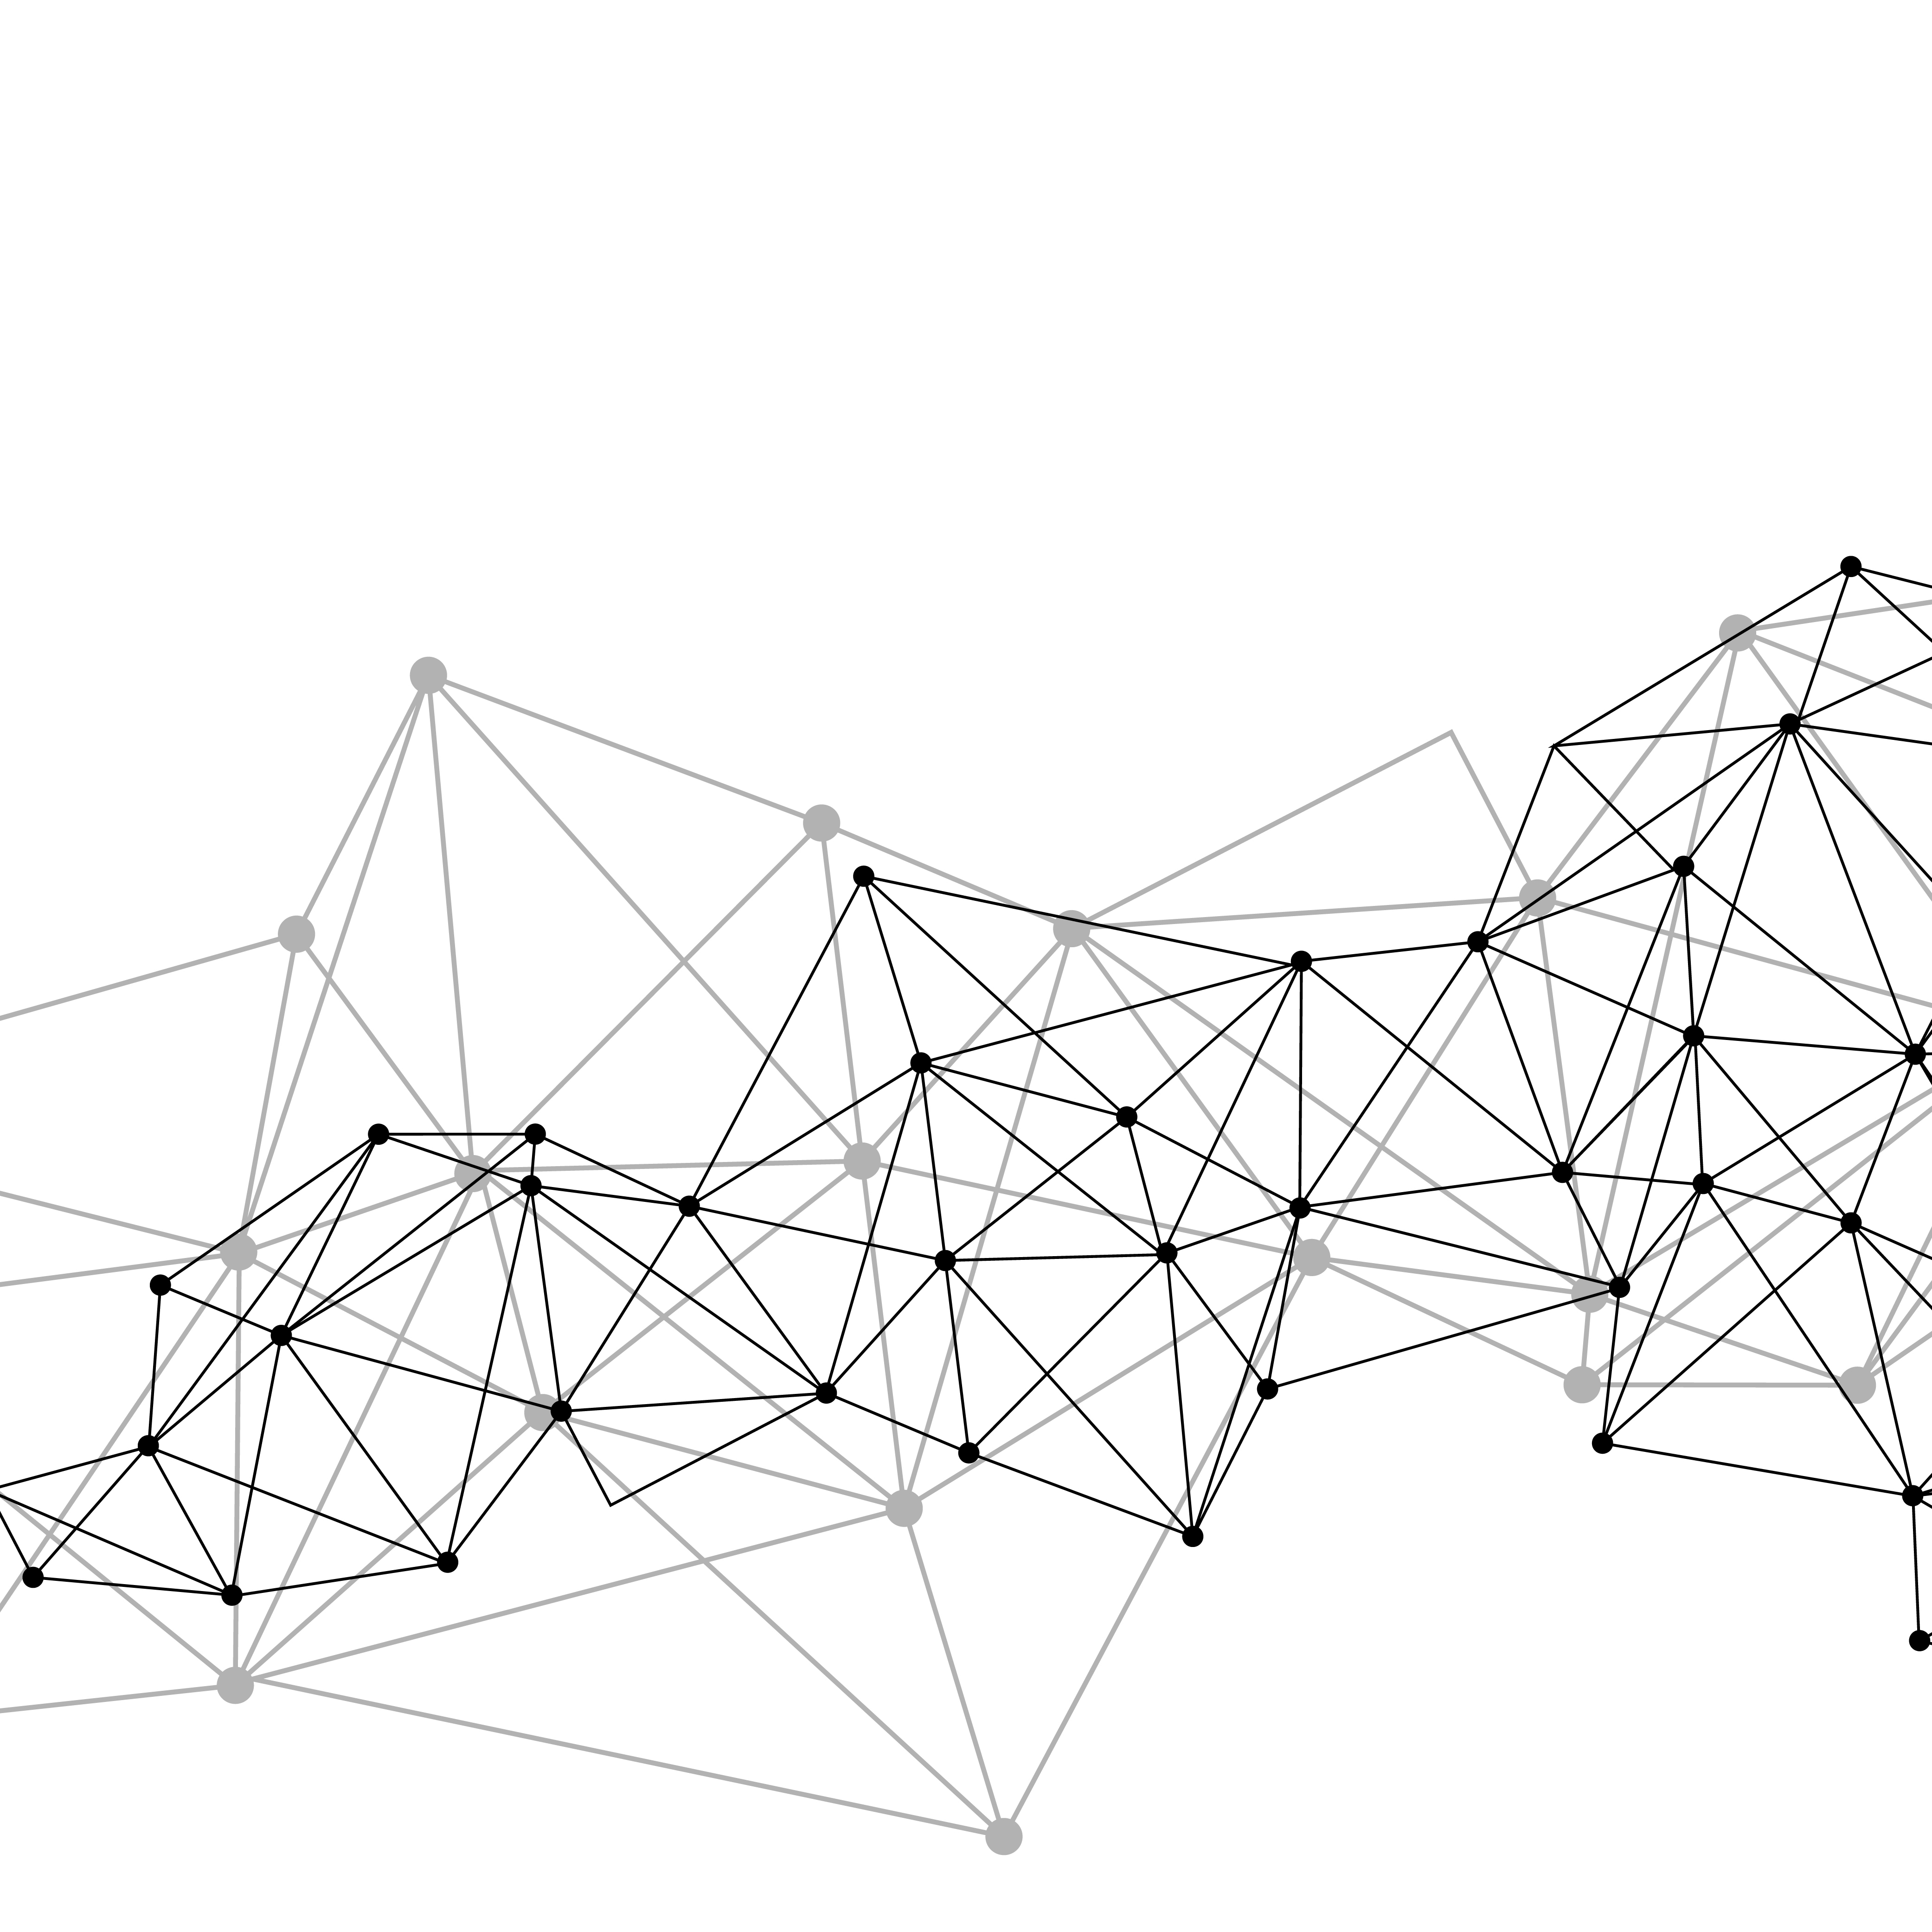
\includegraphics[width=\paperwidth]{img/main-background.jpg} 
  \end{backgroundblock} 
  \titlepage 
\end{frame}
\section{Introduction}
% ! TeX root = ../document.tex
\begin{frame}{ \playfairblack Introduction }
  \begin{card}[Aggregate Computing as a novel approach to \textit{collective computation}]
    \begin{itemize}
      \item[\success{\faThumbsUp}] Aggregate Computing has been grown fastly in the last few years
      \item[\success{\faThumbsUp}] Pulverisation, design patterns, distributed schedulers are prosed to close the ``reality gap"
      \item[\failure{\faThumbsDown}] Some of the building blocks currently have some limitations
      \item[\failure{\faThumbsDown}] The algorithms configuration typically involve a fine-tuning of several parameters
      \item[\failure{\faThumbsDown}] Middleware aspects need a priori knowledge of the application domain
      \item[\highlightAlt{\faLightbulb}] Learning as a mechanism to improve adaptivity by  \emph{experience}
    \end{itemize}
  \end{card}
\end{frame}
\section{Vision}
\begin{frame}{\playfairblack Vision}
  \begin{card}
    
  \end{card}
\end{frame}
\section{Influences}
\begin{frame}{\playfairblack Influences}
  \begin{backgroundblock} 
    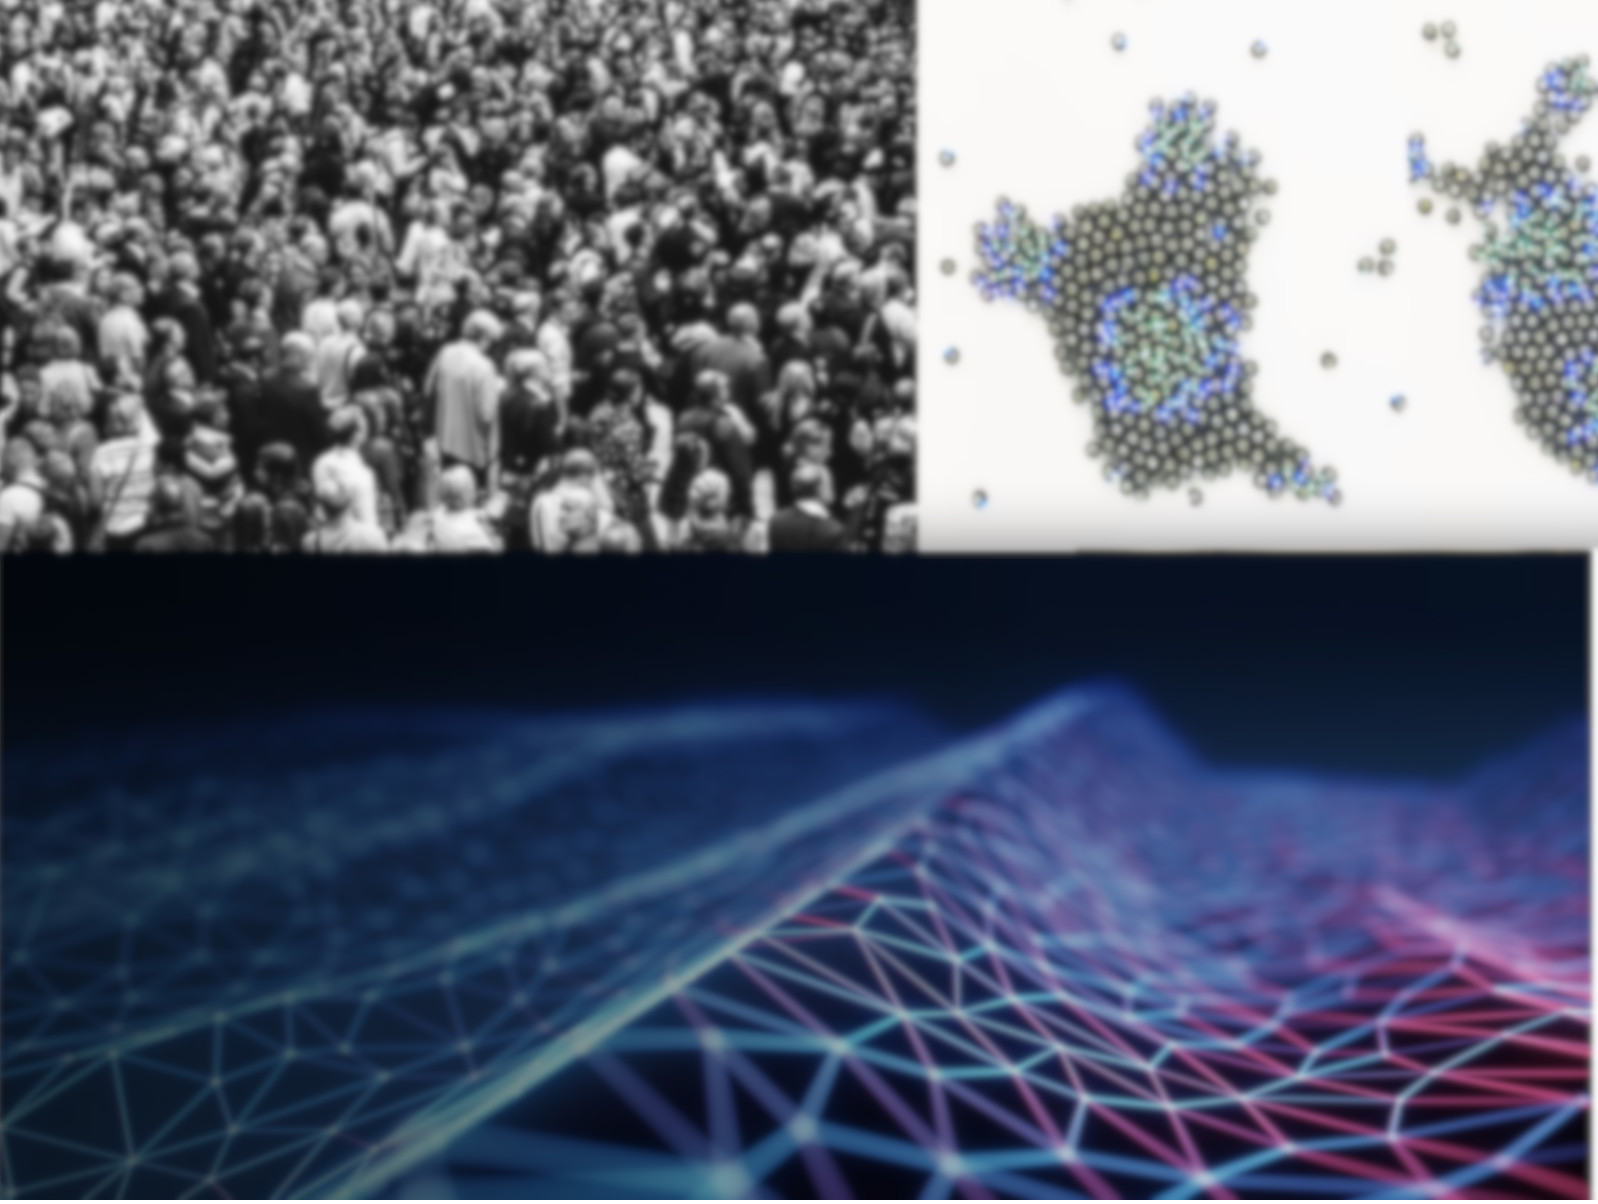
\includegraphics[width=\paperwidth]{img/background} 
  \end{backgroundblock} 
  \begin{card}
    \begin{itemize}
      \item \textbf{Multi Agent Reinforcement Learning}: Reinforcement Learning extension to multiple interacting agents that learn a policy concurrently
      \item \textbf{Graph Neural Networks}: neural networks operating on graphs
      \item \textbf{Mean Field game theory}: game theory extension to a large number of players
      \item \textbf{Swarm Robotics}: large population of robots that exhebits similar behaviours observed in swarm of social animals
    \end{itemize}
  \end{card}
\end{frame}
\section{First attempt}
\begin{frame}{\playfairblack First attempt}
  \begin{card}[RL for improving Hop count program]
    \begin{itemize}
      \item[\failure{\faThumbsDown}] Hop count suffers from the slow rising problem
      \item[\success{\faThumbsUp}] Algorithm solution exists but need a-priori knowledge of the system dynamics
      \item[\highlightAlt{\faLightbulb}] Can we \emph{learn} to speed-up the hop count converge?
    \end{itemize}
  \end{card}
  \begin{columns}[onlytextwidth, t]
    \begin{column}{0.5\textwidth}
      \begin{card}[Hop Count speed up with Hysteric Q-Learning]
        \begin{itemize}
          \item \textbf{State}: velocity of the hop count output
          \item \textbf{Action}: delta correction: \texttt{(1, 2, 3)}
          \item \textbf{Reward}: error from the simulated distance
        \end{itemize}
      \end{card}
    \end{column}
    \begin{column}{0.29\textwidth}
      \cardImg{img/760.pdf}{\textwidth}
    \end{column}
  \end{columns}
\end{frame}
\section{Future works}
% ! TeX root = ../document.tex
\begin{frame}{\playfairblack Future works}
  \begin{backgroundblock} 
    
\includegraphics[width=\paperwidth]{img/conclusion.pdf} 
  \end{backgroundblock} 
  \begin{card}
    \begin{itemize}  
      \item Usage of Deep Learning techniques
      \item Online learning
      \item Focusing on middleware level application
      \item Extend first results to more complicated blocks (e.g. \texttt{S})
    \end{itemize}
  \end{card}
\end{frame}
\end{document}
